% Die folgenden zwei Befehle binden die CoderDojo-Styles ein.
		
\newcommand*{\VorlagenPfad}{../../../../Vorlagen}	
\documentclass{\VorlagenPfad/coderdojokatext}

% Titel als Kommando für den Header/Footer definieren
\newcommand{\Titel}{py2cd - Zeichnen mit Python}
\usepackage{hyperref}

\begin{document}


% Titel anzeigen und um den Header/Footer zu generieren
\begin{center}
	{\huge \Titel}
\end{center}

\section{Vorbereitung}
Um diese Tutorial erfolgreich abzuschließen, muss zuerst pygame und py2cd installiert sein. Eine Anleitung für Windows ist hier \url{https://github.com/coderdojoka/Materialien/raw/master/Installation/installation_pygame.pdf} zu finden.

\section{Einleitung}

\subsection{Koordinaten-System}
Py2cd ist ein 2D-Zeichenframework und folglich wird ein Objekt durch 2 Koordinaten, eine x- und y-Koordinate, festgelegt. Man kann also durch einen Punkt \code{(x|y)} die Position eines Objektes bestimmen.
\begin{merkbox}
\textbf{WICHTIG:} Der Koordinatensystemursprung, also der Punkt \code{(0|0)} liegt in der linken oberen Ecke.
\\Dies ist bei vielen Bildprogrammen wie z.B. Paint oder Gimp genau so.
\end{merkbox}

\subsection{Fenstergröße}
Ein Fenster auf dem Computerbildschirm hat eine bestimmte Größe. Diese Größe wird in Pixeln (px) angegeben. Haben wir bspw. ein Fenster mit der Größe \code{640x480 px},
so sind Objekte, die Koordinaten zwischen \code{x: 0-640 px} und \code{y: 0-480} (zumindest teilweise) sichtbar.

\subsection{Umgebendes Rechteck}
In py2cd sind alle Objekte, also z.B. Kreise, Rechtecke, Bilder von einem 'unsichtbaren' Rechteck umgeben, das das Objekt so genau wie möglich darin einschließt. Dies ist wichtig, da jedes Objekt, auch ein Kreis, so eine Breite und Höhe hat. Diese beiden Werte beziehen sich IMMER auf das umgebende Rechteck. Bei manchen Positionsberechnungen und zur Kollisionserkennung wird dieses Rechteck verwendet. Aus diesem Grund können kleine Ungenauigkeiten auftreten. 

\pagebreak
\section{Ein einfaches Beispiel}
Das folgende Beispiel sollte relativ selbst erklärend sein.
\begin{pythoncode}
# Diese zwei Zeilen werden immer benötigt, um py2cd zu importieren
from py2cd import *
from py2cd.farben import *

# Der erste Schritt um ein Spiel zu starten ist immer,
# der Initialisierungsfunktion init()
Spiel.init(640, 480, "Mein Spiel")
# Erstellt ein neues Fenster mit der gegebenen Größe von 640x480
# und dem Titel 'Mein Spiel'

# ein neues Rechteckt mit Position 270x200 und Größe 100x100 in gelb
haus = Rechteck(270, 200, 100, 100, GELB)

# ein Polygon mit den Ecken aus der Liste und der Farbe Rot
dach = Polygon([(270, 200), (320, 160), (370, 200)], ROT)

# ein neues Rechteck mit Position 320x200 und Größe: 30x50 in grün
tuer = Rechteck(320, 250, 30, 50, GRUEN)

# Eine Linie zwischen den gegeben Punkten in Rot und 2 Pixel dick
boden = Linie((100, 300), (550, 300), ROT, 2)

# Hilfsgitter anzeigen
Spiel.zeichne_gitter()

# Startet das Spiel. Dies muss immer die letze Zeile sein
Spiel.starten()
\end{pythoncode}

\begin{merkbox}
Bevor gezeichnet werden kann muss zuerst py2cd initialisiert werden mit:
\begin{pythoncode}
Spiel.init(640, 480, "Mein Spiel")
\end{pythoncode}
Um das Fenster zu starten, muss dieser Code am Ende eingefügt werden:
\begin{pythoncode}
Spiel.starten()
\end{pythoncode}
\end{merkbox}
\subsection{Weitere Zeichen-Befehle:}
Es gibt noch viele weitere Zeichenbefehle und nützliche Funktionen. Hier noch ein paar weitere aufgezählt.
\subsection{Kreise}
Kreise können ebenfalls ganz einfach gezeichnet werden:
\begin{pythoncode}
# Einen Kreis mit linker Ecke 140x140, einem Radius von 60 px
k = Kreis(140, 140, 60, MATT_GRUEN)
# Die Mitte des Kreises auf 200x200 setzen
k.setze_mitte(200, 200)
\end{pythoncode}

Bei Kreisen ist es meistens sehr umständlich diese über die linke obere Ecke zu positionieren. Deshalb ist es einfacher die Position im nachhin mit der Funktion \code{setze\_mitte(x, y)} zu korrigieren. Auch andere Objekte, wie Rechtecke können mit dieser Funktion positioniert werden.

\subsection{Bilder}
Man kann auch eigene Bilder zeichen lassen:
\begin{pythoncode}
# Das Bild in den BildSpeicher laden und ihm einen Namen geben: 'scratch' 
BildSpeicher.lade_bild("scratch", "scratch.png")
# Das Bild über seinen Namen holen und anzeigen
b = BildSpeicher.gib_bild("scratch")
# Die Position setzen
b.setze_position(50, 20)
\end{pythoncode}
Bilder kann man über den Bildspeicher laden. Dafür müssen sie zuerst geladen werden und können danach über ihren Namen abgerufen werden. Die Postion des Bildes wird nachträglich mit der Funktion \code{setze\_position(x, y)} gesetzt. Diese Funktion steht auch bei anderen Objekten wie Rechtecken und Kreisen zur Verfügung.
\textbf{Hinweis:} Das Bild muss im gleichen Ordner wie dein Programm liegen. Alternativ kannst du auch den Pfad \code{"scratch.png"} ändern.

\subsection{Eigene Farben}
Im Zusammenhang mit Computer und Farben spricht man oft von RGB Farben. RGB steht für Rot, Grün, Blau. Eine Farbe wird also aus 3 Komponenten aufgebaut: Einem Rotanteil, Grünanteil und einem Blauanteil. Die R-, G-, B-Werte dürfen dabei Werte zwischen 0 und 255 annehmen. Die Farbe Schwarz entspricht \code{(0, 0, 0)}, Weiß ist \code{(255, 255, 255)}. 
Willst du nun eine eigene Farbe verwenden kannst du dies einfach als 3-Tupel angaben:

\begin{pythoncode}
meineFarbe = (255, 0, 0) # Rot voll, Grün und Blau nichts => Rot
r = Rechteck(10, 10, 50, 50, meineFarbe)
\end{pythoncode}
Eine Farbe wählst du dir am Besten in einem Bildbearbeitungsprogramm wie Paint, Gimp (oder online) aus. Merke dir die RGB-Werte und füge sie in dein Programm ein.
\section{Aufgaben}
\begin{enumerate}
\item Male einen Apfelbaum, das ganze könnte ungefähr so aussehen:
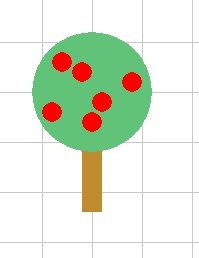
\includegraphics[width=20mm]{baum.png}	
\\\textbf{Hinweis:} Mithilfe des Gitters kannst du die Position der Gegenstände besser ermitteln.

\item Spiele mit den verschiedenen Funktionen herum. Male dein eigenes Bild! Lade eigene Bilder und verändere ihre Position.
\end{enumerate}

\end{document}